\documentclass[11pt]{article}
\usepackage[margin=2.2cm]{geometry}
\usepackage{tikz}
\begin{document}
\section*{Structural-completeness recount (sheriff case SHF-20261016-3caa6f)}
The paper's ``16\,562 ordinary curve instances'' matched no script output.
Re-running the cited scripts (logs in this directory, \texttt{count.py})
gives the counts below. Every ordinary instance in the lemma's hypothesis
class satisfies it (0 violations); the excluded class $r=\ell-1$ always has
$\ell \mid \#E^t$, as predicted. The CM-73 sweep processed the 330 primes
$p \equiv 1 \pmod 6$, $7 \le p \le 5000$ (not 621).

\begin{center}\begin{tabular}{rrrrr}
$\ell$ & ordinary, hypothesis & ordinary, excluded & supersingular & total\\\hline
3 & 5,250 & 0 & 10,938 & 16,188 \\
5 & 315 & 0 & 3,096 & 3,411 \\
7 & 2,591 & 578 & 1,708 & 4,877 \\
11 & 198 & 0 & 0 & 198 \\
13 & 1,510 & 94 & 0 & 1,604 \\
\hline
all & 9,864 & 672 & 15,742 & 26,278
\end{tabular}\end{center}

\begin{center}
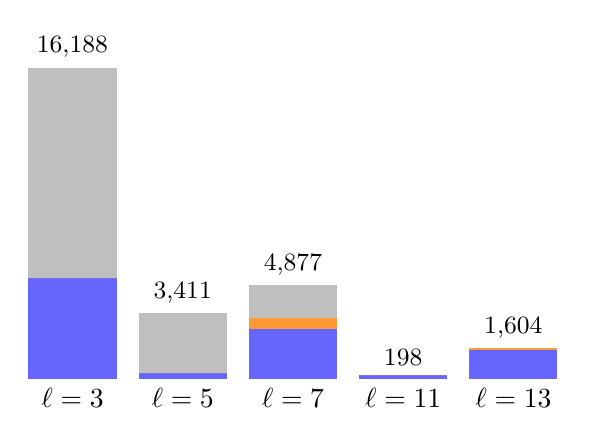
\begin{tikzpicture}[x=1.4cm,y=0.00025cm]
\fill[blue!60] (0,0) rectangle (0+0.8,5250);\fill[orange!80] (0,5250) rectangle (0+0.8,5250);\fill[gray!50] (0,5250) rectangle (0+0.8,16188);\node[below] at (0+0.4,0) {$\ell=3$};\node[above] at (0+0.4,16188) {\small 16,188};
\fill[blue!60] (1,0) rectangle (1+0.8,315);\fill[orange!80] (1,315) rectangle (1+0.8,315);\fill[gray!50] (1,315) rectangle (1+0.8,3411);\node[below] at (1+0.4,0) {$\ell=5$};\node[above] at (1+0.4,3411) {\small 3,411};
\fill[blue!60] (2,0) rectangle (2+0.8,2591);\fill[orange!80] (2,2591) rectangle (2+0.8,3169);\fill[gray!50] (2,3169) rectangle (2+0.8,4877);\node[below] at (2+0.4,0) {$\ell=7$};\node[above] at (2+0.4,4877) {\small 4,877};
\fill[blue!60] (3,0) rectangle (3+0.8,198);\fill[orange!80] (3,198) rectangle (3+0.8,198);\fill[gray!50] (3,198) rectangle (3+0.8,198);\node[below] at (3+0.4,0) {$\ell=11$};\node[above] at (3+0.4,198) {\small 198};
\fill[blue!60] (4,0) rectangle (4+0.8,1510);\fill[orange!80] (4,1510) rectangle (4+0.8,1604);\fill[gray!50] (4,1604) rectangle (4+0.8,1604);\node[below] at (4+0.4,0) {$\ell=13$};\node[above] at (4+0.4,1604) {\small 1,604};
\end{tikzpicture}

\small blue: ordinary, hypothesis class; orange: ordinary, $r=\ell-1$; grey: supersingular.
\end{center}
\end{document}
